% tikzpic.tex
\documentclass[crop,tikz]{standalone}% 'crop' is the default for v1.0, before it was 'preview'
%\usetikzlibrary{...}% tikz package already loaded by 'tikz' option
\usepackage{amsmath,amsthm,amssymb,mathrsfs,amsfonts,dsfont}

\begin{document}
    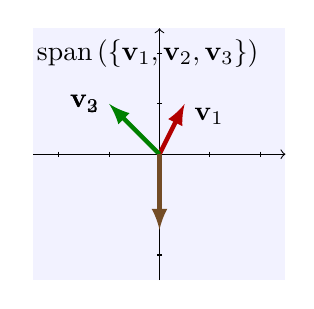
\begin{tikzpicture}[scale=0.32]
        % Fill the entire R2 space with light blue color
        \fill[blue!5] (-5,-5) rectangle (5,5);

        \draw[->, thin, black] (-5,0) -- (5,0);
        \draw[->, thin, black] (0,-5) -- (0,5);
        \foreach \x in {-4,-2,2,4}
        \draw (\x,0.1) -- (\x,-0.1);
        \foreach \y in {-4,-2,2,4}
        \draw (0.1,\y) -- (-0.1,\y);

        \node[black, xshift=-0.15cm] at (0, 4) {$\text{span}\left(\left\{\mathbf{v}_1, \mathbf{v}_2, \mathbf{v}_3\right\}\right)$};
        
        \draw[-latex, ultra thick, red!70!black] (0, 0) --  (1,2);
        \node[right, black] at (1.0, 1.5) {$\mathbf{v}_1$};
        
        \draw[-latex, ultra thick, green!50!black] (0, 0) --  (-2,2);
        \node[left, black] at (-2, 2) {$\mathbf{v}_2$};
        
        \draw[-latex, ultra thick, brown!60!black] (0, 0) --  (0,-3);
        \node[left, black] at (-2, 2) {$\mathbf{v}_3$};
    \end{tikzpicture}
\end{document}